\section{Necessary concepts}

Before analysing the problem and the existing works on the topic and before describing the hardware used and the data captured, it is worth explaining some of the concepts behind SDR and NFC. We will only discuss the elements needed to understand this document, and will refer the reader to other works for details. Readers that are acquainted to software-defined radio and NFC's characteristics can skip this section and continue at section \ref{sota}.

\subsection{Software-defined radio}

First, we will note that radio waves are electromagnetic radiations operating in the Radio Frequency (RF) range. RF is a portion of the electromagnetic spectrum generally comprised between $\sim$3kHz and 300GHz \cite{pritchard_elttam}. It is used for radio communications of all sorts.

The main principle behind software-defined radio, as its name suggests, is to make as many of the elements of a traditional radio's pipeline digital. Doing this makes it possible to use a computer's processor to do the signal processing tasks that once required specialized hardware. Of course, it is not functional to simply strap an antenna to an Analog-to-Digital Converter (ADC) and do everything else in software. We still need some analog components in front of the ADC to preprocess the signal and ensure a consistent sampling. \cite{wiki_software-defined_2020, hackaday_your_2015, spiess_286_2019}

These analog components are combined in SDR hardware available to buy. Popular examples include the cheap RTL-SDR dongle\footnote{\url{https://www.rtl-sdr.com/about-rtl-sdr}} (receiver) and the HackRF\footnote{\url{https://greatscottgadgets.com/hackrf/one}} (transceiver). Once an SDR is plugged into a computer, the proper drivers and software are installed and an antenna is connected to the device, anybody is able to receive and process a wide range of frequencies. This range is limited by the components in the SDR hardware and by the antenna.

\begin{figure}[htp!]
  \centering
  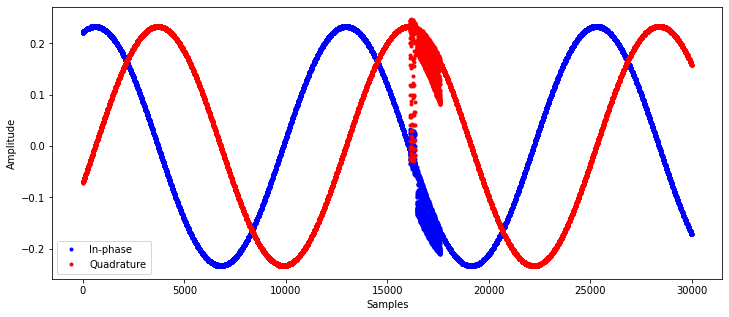
\includegraphics[scale=0.5]{figures/concepts_IQ-signal.png}
  \caption{In-phase and quadrature components of a signal}
  \label{fig:iq-signal}
\end{figure}

To finish this introduction to SDR, we will describe the representation of the data. Figure \ref{fig:iq-signal} shows a graph of the samples returned by the SDR pipeline as dots. As can be seen, the signal is represented using two components. The "quadrature" component is phase shifted by 90 degrees in relation to the "in-phase" component. Every sample can be represented by a complex number where the real part adds to the in-phase component and the imaginary part adds to the quadrature component. Such a representation allows us to get a lot more information from the signal. \cite{kuisma_iq, ossmann_software}

Here, the X axis represents the sample number (starting at 0) rather than a time value. The link between the sample number and the time elapsed is the sampling rate ($F_s$), expressed in number of samples per second (S/s). For example, considering a sampling rate of 3MS/s, figure \ref{fig:iq-signal} shows a signal over 10ms: $\dfrac{30000[S]}{3000000[S/s]} = 0.01[s]$.

In this document, we will often use the magnitudes representation of a signal. Said representation is built by taking the magnitude (or module) of each complex sample and plotting it. Figure \ref{fig:mag} shows the magnitudes of the samples in figure \ref{fig:iq-signal}.

\begin{figure}[htp!]
  \centering
  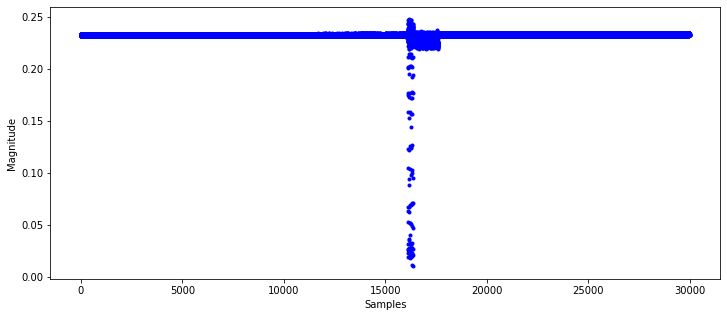
\includegraphics[scale=0.5]{figures/concepts_magnitudes.png}
  \caption{A signal represented as the magnitudes of its samples}
  \label{fig:mag}
\end{figure}

% -------------------------------------------------------------------------------------------------------------
\subsection{Near-field communication} \label{nfc}

In order for our radio system to be effective, it needs to be adapted to the protocols used. This is why we need to understand how NFC operates.

NFC is the name for a group of communication protocols designed for small distance (max. 10cm) transactions. The idea is that a reader can supply power to a passive tag and get the information stored in it. The reader devices are sometimes called initiators or PCD (for Proximity Coupling Device) and the tags are sometimes called targets or PICC (for Proximity Inductive Coupling Card).

Operating at a frequency of 13.56MHz, NFC is well in the High Frequency (HF) range of 3 to 30MHz. This is substantially lower than most communication protocols like WiFi (2.4GHz or 5GHz), Bluetooth (2.4GHz) or ZigBee (868MHz, 915MHz or 2.4GHz).

Also in contrast to these other protocols, NFC's modulation scheme is On-Off Keying (OOK) which is a form of Amplitude Shift Keying (ASK). (Except for NFC type B, which uses Binary Phase Shift Keying (BPSK) in target to initiator mode.)

Because it is designed to work only in close proximity, NFC uses inductive coupling between devices to transmit information. In simple terms, this means the reader can only send a signal as far as its generated magnetic field goes. The passive tag responds by modulating the same magnetic field. It also means that far-field interferences from radio devices operating in the same frequency range practically don't affect an NFC communication. \cite{wiki_near-field_2020}
